\expandafter\let\csname ver@amssymb.sty\endcsname\empty
\documentclass[serif]{beamer}
\expandafter\let\csname ver@amssymb.sty\endcsname\relax
\usepackage{etex}
\usepackage[bitstream-charter]{mathdesign} % Use BT Charter font
\usepackage[T1]{fontenc}                   % Use T1 encoding instead of OT1
\usepackage[utf8]{inputenc}                % Use UTF8 input encoding
\usepackage{microtype}                     % Improve typography
\usepackage{booktabs}
\usepackage{cancel}
\usepackage{algorithm}
\usepackage{algorithmicx}
\usepackage{algpseudocode}
\usepackage{hyperref}
\hypersetup{pdfstartview=Fit}
\usepackage{tikz}
\usetikzlibrary{shapes,snakes,shadows,arrows,calc}
\usetikzlibrary{decorations.markings}
\usepackage{multirow}
\usepackage{animate}
\usepackage{moresize}
\usepackage{colortbl}
\usepackage{xcolor}
\usepackage{amsmath}
\usepackage{etoolbox}
\usepackage{listings}
\usepackage{alltt}
\usepackage{textpos}

\renewcommand\footnotemark{}

\lstset{
  basewidth=0.5em,
%  columns=fullflexible,
  showspaces=false,
  showtabs=false,
  showstringspaces=false,
  commentstyle=\color{gray}\upshape,
}
\lstdefinelanguage{XML}
{
  backgroundcolor=\color{gray!20},
  basicstyle=\ttfamily\ssmall,
  morestring=[b]",
  frame=single,
% morestring=[s]{>}{<},
  morecomment=[s]{<?}{?>},
  morecomment=[s]{<!--}{-->},
  stringstyle=\color{red},
  identifierstyle=\color{darkblue},
  keywordstyle=\color{cyan},
}

\definecolor{gray}{rgb}{0.4,0.4,0.4}
\definecolor{darkblue}{rgb}{0.0,0.0,0.6}
\definecolor{cyan}{rgb}{0.0,0.6,0.6}

\newcommand{\tikzmark}[1]{\tikz[overlay,remember picture] \node (#1) {};}
\newcommand*{\DrawArrow}[3][]{%
    % #1 = draw options
    % #2 = left point
    % #3 = right point
    \begin{tikzpicture}[overlay,remember picture]
        \draw [-latex, #1] ($(#2)+(0.3em,-1ex)$) to ($(#3)+(0,0.5ex)$);
    \end{tikzpicture}%
}

\usetheme{Copenhagen}
\usecolortheme{beaver}

\title{OpenMC Module: Tally Specification and Data Extraction}
\author{\emph{Computational Reactor Physics Group}}
\date{\normalsize Department of Nuclear Science and Engineering\\
                  Massachusetts Institute of Technology \\
~\\
\tiny{This work is licensed under the Creative Commons Attribution-ShareAlike 3.0 Unported License. To view a copy of this license, visit http://creativecommons.org/licenses/by-sa/3.0/.}}

% Set Logo
\logo{
\includegraphics[scale=0.2]{src/crpg.png}\hspace*{8cm}

\includegraphics[scale=0.2,trim=0cm 3.0cm 2.2cm 0cm, clip=true]{src/mitlogo.pdf}}

\usenavigationsymbolstemplate{}

%-------------------------------------------------------------------------------
\begin{document}
%-------------------------------------------------------------------------------

\frame{\titlepage}\logo{} % remove logo after title page


%-------------------------------------------------------------------------------

\begin{frame}{How Do We Get Results?}

  \centering
  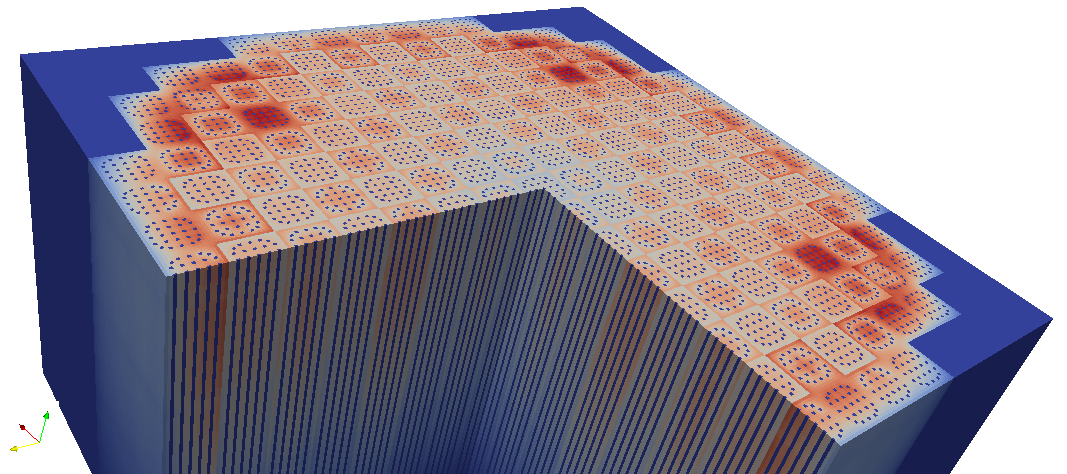
\includegraphics[width=\linewidth]{src/3dcore.png}

\end{frame}

%-------------------------------------------------------------------------------

\begin{frame}{Tallying Physics}

  \begin{itemize}
    \item Method to extract quantities out of Monte Carlo run (e.g., flux, reaction rates, current, etc.)\vfill
    \item Tallies are made using different estimators (e.g., analog, collision, track-length)\vfill
    \item When an event occurs, the following formula is used for tallies:
\[
      {\rm{tally}} = \sum_{i\in\rm{events}}\frac{R_iw_i\phi_i}{W}
\]\vfill
    \item $w_i$: neutron statistical weight, where $W$ is total starting weight
    \item $R_i$: response function (flux=1, reaction rates=$\Sigma$)
    \item $\phi$: estimator (analog=1, collision=$\Sigma_t^{-1}$, track=$d$)
  \end{itemize}

\end{frame}

%-------------------------------------------------------------------------------

\begin{frame}[fragile]{Tally Specifications in OpenMC}

  \begin{itemize}
    \item Tallies are specified on \verb|tallies.xml|
    \begin{itemize}
      \item See xml files in examples/demos/tallying
    \end{itemize}
    \item Each tally has \textit{scores} and \textit{filters}
    \begin{itemize}
      \item \textit{Scores} specify \underline{what} to tally
      \item \textit{Filters} specify \underline{where} to tally
    \end{itemize}
    \item Can choose tally estimator type: analog, tracklength, collision
  \end{itemize}

  \begin{scriptsize}
    \begin{lstlisting}[language=XML,gobble=4]
    <?xml version="1.0" encoding="UTF-8"?>
    <tallies>

      <tally id="1">
        <label>My Tally Label</label>
        <filter type="cell" bins="10 20 30"/>
        <scores>flux</scores>
        <estimator>tracklength</estimator>
      </tally>
      
    </tallies>
    \end{lstlisting}
  \end{scriptsize}

\end{frame}

%-------------------------------------------------------------------------------

\begin{frame}[fragile]{Tally Scores}

  \begin{itemize}
    \item Multiple responsed can be scored at the same time
    \item 
  \end{itemize}

flux:           Total flux
total:          Total reaction rate
scatter:        Total scattering rate. Can also be identified with the scatter-0 response type.
nu-scatter:     Total production of neutrons due to scattering. This accounts for multiplicity from (n,2n), (n,3n), and (n,4n) reactions and should be slightly higher than the scattering rate.
scatter-N:      Tally the Nth scattering moment, where N is the Legendre expansion order. N must be between 0 and 10. As an example, tallying the 2nd scattering moment would be specified as <scores> scatter-2 </scores>.
scatter-PN:     Tally all of the scattering moments from order 0 to N, where N is the Legendre expansion order. That is, scatter-P1 is equivalent to requesting tallies of scatter-0 and scatter-1. N must be between 0 and 10. As an example, tallying up to the 2nd scattering moment would be specified as <scores> scatter-P2 </scores>.
absorption:     Total absorption rate. This accounts for all reactions which do not produce secondary neutrons.
fission:        Total fission rate
nu-fission:     Total production of neutrons due to fission
kappa-fission:  The recoverable energy production rate due to fission. The recoverable energy is defined as the fission product kinetic energy, prompt and delayed neutron kinetic energies, prompt and delayed -ray total energies, and the total energy released by the delayed  particles. The neutrino energy does not contribute to this response. The prompt and delayed -rays are assumed to deposit their energy locally.
events:         Number of scoring events

  \begin{scriptsize}
    \begin{lstlisting}[language=XML,gobble=4]

    \end{lstlisting}
  \end{scriptsize}

\end{frame}

%-------------------------------------------------------------------------------

\begin{frame}[fragile]{Tally Filters}

  \begin{itemize}
    \item 
    \item 
  \end{itemize}

cell:       A list of cells in which the tally should be accumulated.
cellborn:   This filter allows the tally to be scored to only when particles were originally born in a specified cell.
surface:    A list of surfaces for which the tally should be accumulated.
material:   A list of materials for which the tally should be accumulated.
universe:   A list of universes for which the tally should be accumulated.
energy:     A monotonically increasing list of bounding pre-collision energies for a number of groups. For example, if this filter is specified as <energy>0.0 1.0 20.0</energy>, then two energy bins will be created, one with energies between 0 and 1 MeV and the other with energies between 1 and 20 MeV.
energyout:  A monotonically increasing list of bounding post-collision energies for a number of groups. For example, if this filter is specified as <energyout>0.0 1.0 20.0</energyout>, then two post-collision energy bins will be created, one with energies between 0 and 1 MeV and the other with energies between 1 and 20 MeV.
mesh:       The id of a structured mesh to be tallied over.


  \begin{scriptsize}
    \begin{lstlisting}[language=XML,gobble=4]

<nuclides>U-235 total</nuclides>

    \end{lstlisting}
  \end{scriptsize}

\end{frame}


%-------------------------------------------------------------------------------

\begin{frame}[fragile]{Tallies Are Set, OpenMC is Run -- Now What?}

  \begin{itemize}
    \item The manual way: Look at tallies.out
  \end{itemize}

  \begingroup
    \centering
    \fontsize{4pt}{4.8pt}\selectfont
    \begin{semiverbatim}
 ===================>     TALLY 1: MY TEST TALLY #1     <===================

 Mesh Index (1, 1, 1)
   Incoming Energy [0.0, 6.25000E-07)
     Total Material
       Flux                        0.0            +/- 0.0
  ...
  ...
 Mesh Index (24, 15, 3)
   Incoming Energy [0.0, 6.25000E-07)
     Total Material
       Flux                        7.42110E-08    +/- 3.14470E-08
   Incoming Energy [6.25000E-07, 20.0000)
     Total Material
       Flux                        2.07275E-07    +/- 6.29534E-08
 Mesh Index (24, 15, 4)
   Incoming Energy [0.0, 6.25000E-07)
     Total Material
       Flux                        1.20947E-07    +/- 6.08719E-08
   Incoming Energy [6.25000E-07, 20.0000)
     Total Material
       Flux                        1.39299E-07    +/- 4.56898E-08
 Mesh Index (24, 15, 5)
   Incoming Energy [0.0, 6.25000E-07)
     Total Material
  ...
  ...
      
    \end{semiverbatim}
  \endgroup

\end{frame}

%-------------------------------------------------------------------------------

\begin{frame}[fragile]{Tallies Are Set, OpenMC is Run -- Now What?}

  \begin{itemize}
    \item The Better Way$\texttrademark$: Parse statepoint files
    \item Run OpenMC to generate statepoint files
    \begin{itemize}
      \item Statepoints can be generated at any time throughout the run with the
      \verb|<state_point>| tag in the \verb|settings.xml|
    \end{itemize}
    \item Use the \verb|statepoint.py| utility to parse them
    \begin{itemize}
      \item Once in python, it's easy to output to anything you want
    \end{itemize}
  \end{itemize}

\end{frame}

%-------------------------------------------------------------------------------

\begin{frame}[fragile]{Using Statepoint.py}

  \begin{itemize}
    \item Located in the src/utils directory of the OpenMC source
    \item Provides a simple user front-end for extracting tally data from
    statepoint files
  \end{itemize}

  \begin{scriptsize}
    \begin{lstlisting}[language=Python,backgroundcolor=\color{gray!20},frame=single]
    sp = statepoint.StatePoint('statepoint.300.binary')
    sp.read_results()
    
    for tally in sp.tallies:
        print tally.id
        print tally.scores
        print tally.filters

    print sp.meshes
    \end{lstlisting}
  \end{scriptsize}

\end{frame}

%-------------------------------------------------------------------------------

\begin{frame}[fragile]{Using Statepoint.py}

  \begingroup
    \fontsize{5pt}{5.8pt}\selectfont
    \begin{lstlisting}[language=Python,backgroundcolor=\color{gray!20},frame=single]
    tallyid = 0
    scoreid = 0
    egroupid = 0
    values = {}
    for x in range(1,nx+1):
        for y in range(1,ny+1):
            for z in range(1,nz+1):
                val,err = sp.get_value(tallyid,
                                       [('mesh',(x,y,z)),('energying',energyid)],
                                       scoreid)
                values[(x,y,z)] = val
    \end{lstlisting}
  \endgroup
      
  \centering
  
  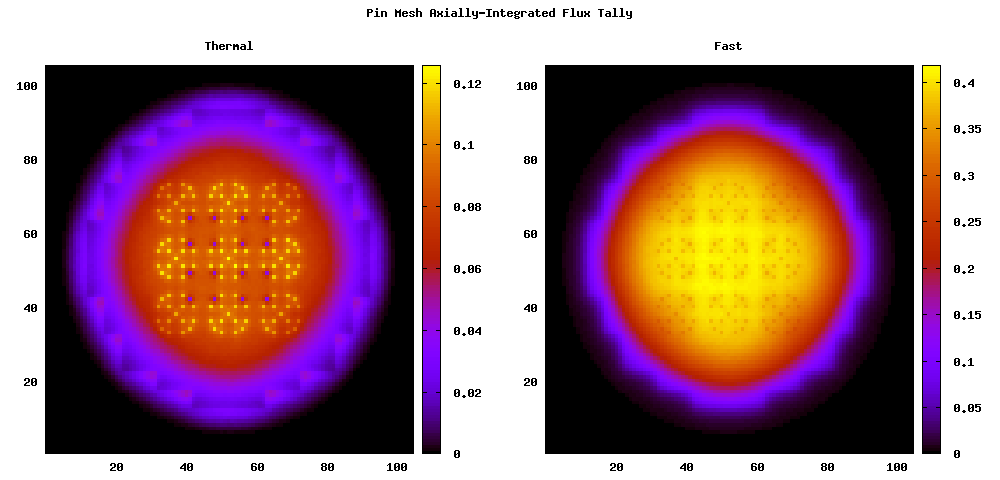
\includegraphics[width=4in]{src/fluxplot.png}

  \setlength{\TPHorizModule}{\framewidth}
  \setlength{\TPVertModule}{\paperheight}
  \begin{textblock}{1}(0.1,-0.75)
    See parse.py in examples/demos/tallying
  \end{textblock}

\end{frame}

%-------------------------------------------------------------------------------

\begin{frame}{Questions?}

  \centering
  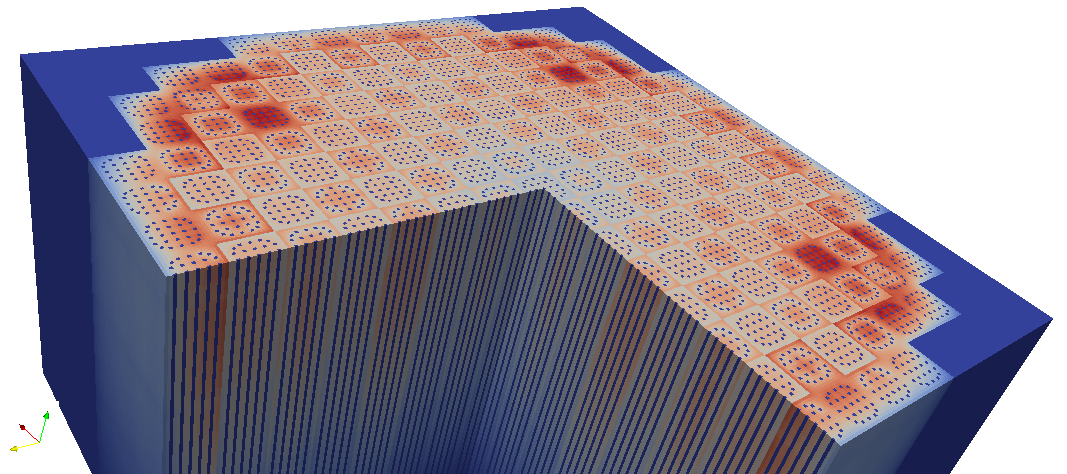
\includegraphics[width=\linewidth]{src/3dcore.png}
      
\end{frame}


%basics
%filters
%scores
%output and processing
%  text output
%  statepoints

%-------------------------------------------------------------------------------
\end{document}
%-------------------------------------------------------------------------------
